
\section{Methodology} 

In this cost report, we draw on three major reports that summarize the cost categories for a power plant, based on the methodology developed first by the IAEA, then by the GENIV Economics Modeling Working Group (G4EMWG), and by the lead of the G4EMWG. Geoffrey Rothwell, in his book 'Economics of Nuclear Power'.  There is purposeful use of existing well-documented and contemporary cost basis methodologies represented in these reports, as this documentation will assist anyone who wishes to perform similar analysis.\\

The cost categories depart from prior fusion costing studies by breaking the direct costs into categories 10 (pre-construction) and 20 (construction) and the indirect costs into categories 30-60 (formerly 91-98).  There are some major similarities (in 20, for example, they are almost exactly the same, except for inclusion of a digital twin and contingency), and there are minor variations of the categories that make a lot more sense, for example decommissioning costs are included as a capitalized indirect cost rather than added somewhat obscurely to the LCOE, allowing deeper discussion of the contributing costs to decommissioning.  In this section we describe the main texts that are foundational to the methodology and also those that provide information on cost basis.  Fusion systems of course depart significantly from those of fission in the heat island, fuel cycle, handling, and replacement schedule of major cost components - those are spelled out in each section.  We adopt the subcategory descriptions of most of the GENIV subcategories, but have edited those to more narrowly capture the fusion system costs.\\  

Our philosophy has been to provide recent cost basis information for all cost categories, and state those in the text, providing a reference to the cost basis, and any other reference that will assist the user of the code.  We have also tried to be judicious in our use of terminology: at the time of writing, the term `reactor' is still viewed unfavorably and it's continued use may cause hurdles in the adoption of fusion energy systems, so we have replaced with `heat island'.  For old hands, and those in the nuclear sector, this change in terminology may seem to be superficial, since currently there is renewed interest in nuclear power as a solution for climate mitigation.  We will evolve the terms as necessary, but for this edition, we try to be consistent in the use of terminology that conveys function without connotations.

\begin{figure}[h!] 
\centering 
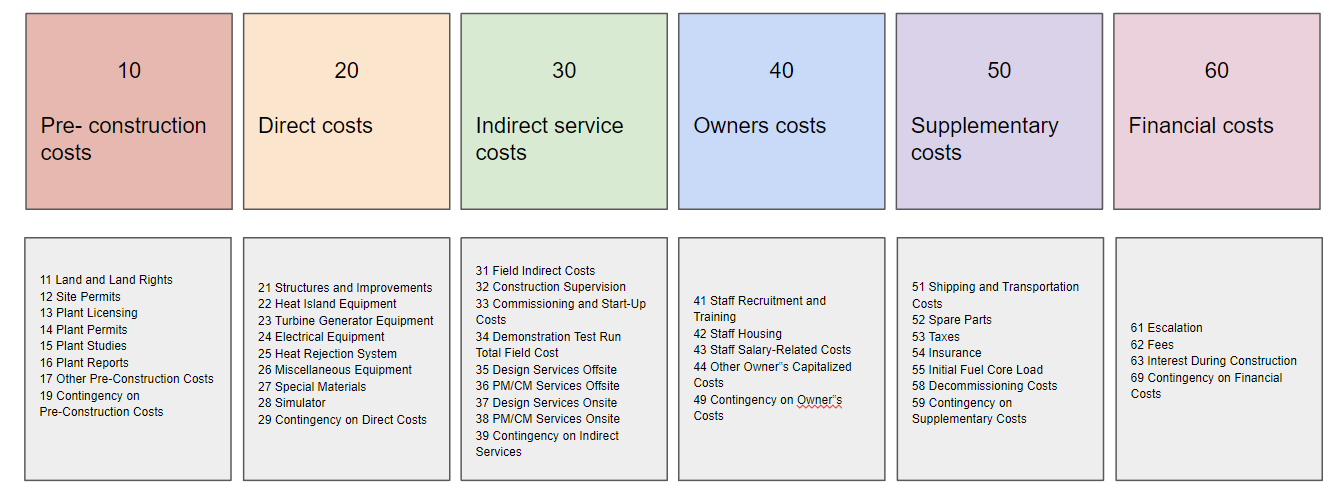
\includegraphics[scale=0.45]{{StandardFigures/costcategories.png}} 
\caption{Cost categories outlined below} 
\label{fig:costcategories} 
\end{figure}

\subsection{Documents influencing the costing methodology}

The GENIV Economics Modeling Working Group (G4EMWG) Guidelines \cite{EMWGOGIIF2007} is a comprehensive guide providing detailed guidelines for economic modeling within the context of Generation IV nuclear energy systems. It systematically outlines the structure for cost estimation, covering various cost categories ranging from pre-construction costs to annualized financial costs. These include detailed breakdowns for capitalized costs (like direct costs, indirect service costs, owner’s costs, and supplementary costs), as well as operational and maintenance costs, fuel costs, and financial costs. The document is meticulously organized, offering a granular view of each cost component, including land rights, permits, licensing, structures, equipment, and contingency costs. It serves as an essential resource for accurately assessing the economic feasibility and overall budgeting for advanced nuclear power plant projects. The guidelines emphasize the importance of detailed cost accounting for ensuring financial viability and strategic planning in the nuclear energy sector.\\

The book "The Economics of Future Nuclear Power", by Geofrey Rothwell \cite{Rothwell2015}, is a comprehensive analysis of the economic factors influencing the future of nuclear power.  The document broadly delves into various aspects such as cost estimation, risk aversion, and capital cost determination for nuclear power projects. It discusses the intricacies of financial modeling and risk assessment, emphasizing the importance of accurately gauging uncertainties and potential costs associated with nuclear energy development. The text also explores the concept of risk diversification, applying financial market theories to the realm of nuclear power investment and development. The content is quite technical, focusing on economic and financial theories as they apply to the nuclear power industry, with detailed mathematical and statistical analyses to support its discussions.\\

The IAEA Tecdoc TRS396 \cite{Meyer2000} is a technical report by the International Atomic Energy Agency (IAEA), providing comprehensive guidelines and methodologies for economic evaluation in the nuclear power sector. The report delves into the economic analysis of nuclear power plants, offering detailed methods for calculating the Levelized Discounted Electricity Generation Costs (LDEGC). It incorporates a range of financial aspects including capital investment costs, operation and maintenance costs, and nuclear fuel cycle costs. The report also discusses the significance of various economic parameters such as discount rates, inflation, and escalation rates in the assessment of nuclear power projects. Additionally, it offers insights into sensitivity analysis, which is crucial for understanding the impact of varying economic conditions on project viability. The document is a valuable resource for professionals in the nuclear industry, providing a structured approach to evaluating the economic feasibility of nuclear power projects.

\subsection{Documents providing cost bases}

The UCSD Report titled "ARIES Cost Account Documentation" by L. M. Waganer, dated June 2013, from the University of California San Diego's Center for Energy Research \cite{Waganer2013}, is a comprehensive documentation of the ARIES Cost Account. Its purpose is to document the historical economic basis for the ARIES Systems Code costing analyses and develop an updated economic model for future systems studies. It provides a thorough background on previous fusion studies' costing information, detailing conceptual designs and cost data from projects like Starfire, Generomak, and various Inertial Fusion Energy (IFE) designs. The report discusses the importance of historical cost escalation, explaining how past estimates are adjusted to current economic conditions using factors like the U.S. GDP Implicit Price Deflator. It also revisits the general cost account information, originally defined by DOE through the Pacific Northwest Laboratory, and covers various aspects such as spare parts, contingency, and Level of Safety Assurance (LSA) in cost estimation. The document offers a detailed analysis of direct and indirect capital costs, elaborating on each cost account with respect to fusion power plants and their respective costing algorithms, adjustments, and recommendations.\\

The presentation titled "Progress On Cost Modeling - Cost Accounts 20 and 21" by L. M. Waganer, dated 14-15 June 2007 \cite{Waganer2007} is centered on the ARIES Project and focuses on improving and updating cost modeling for fusion power plant designs. It discusses the need for revising the ARIES systems code cost modeling, originally based on models from the early 1990s, due to lack of extensive documentation and limited depth in published cost data. The document highlights various cost accounts, like Cryogenic Cooling, Radioactive Waste Treatment, and Reactor Plant Maintenance Equipment, and stresses the necessity for their detailed documentation. The presentation also touches upon general costing ground rules, safety assurance levels, and provides recommendations for defining and reporting cost accounts with reasonable depth. It includes specific details about costs related to land rights, structures, and site facilities for a fusion power plant, proposing updated cost estimates and methodologies for more accurate and comprehensive financial planning in the context of advanced nuclear fusion research.\\

The document "NETL Cost and Performance Baseline for Fossil Energy Plants Volume 1: Bituminous Coal and Natural Gas to Electricity" \cite{JamesCorrespondingAuthor2019} provides an independent assessment of the cost and performance of selected fossil energy power systems. These systems include Integrated Gasification Combined Cycle (IGCC), Pulverized Coal (PC), and Natural Gas Combined Cycle (NGCC) plants. The assessment is conducted using a systematic, transparent technical, and economic approach. This report is the first in a four-volume series, each addressing different aspects of fossil fuel-based power generation. It plays a critical role in assessing and determining technology combinations for future power markets, offering insights for technology comparisons, and providing a framework for regulators and policymakers. In total, nineteen power plant configurations are analyzed, including various IGCC configurations with and without CO2 capture, PC power plant configurations both subcritical and supercritical with varying levels of CO2 capture, and NGCC power plant configurations with state-of-the-art combustion turbines, again with varying levels of CO2 capture.

\subsection{Prior related costing studies}

ARIES, Sheffield, other MFE studies (already in verbose review).


